% \documentclass{article}
% \usepackage{tikz}
% \usepackage[active,tightpage]{preview}
%\PreviewEnvironment{tikzpicture}
%\setlength\PreviewBorder{7pt}
\definecolor{lavander}{cmyk}{0.2,0.2,0.2,0}
\definecolor{violet}{cmyk}{0.7,0.70,0.7,0}
\definecolor{burntorange}{cmyk}{0.4,0.4,0.4,0}

\def\lav{lavander!90}
\def\oran{orange!30}

\tikzstyle{peers}=[draw,circle,violet,bottom color=lavander,
                  top color= white, text=violet,minimum width=10pt]
\tikzstyle{superpeers}=[draw,circle,burntorange, left color=burntorange,
                       text=violet,minimum width=20pt]
\tikzstyle{legendsp}=[rectangle, draw, burntorange, rounded corners,
                     thin,bottom color=burntorange, top color=white,
                     text=violet, minimum width=2.5cm]
\tikzstyle{legendp}=[rectangle, draw, violet, rounded corners, thin,
                     bottom color=lavander, top color= white,
                     text= violet, minimum width= 2.5cm]
\tikzstyle{legend_general}=[rectangle, rounded corners, thin,
                           burntor\lavange, fill= white, draw, text=violet,
                           minimum width=2.5cm, minimum height=0.8cm]

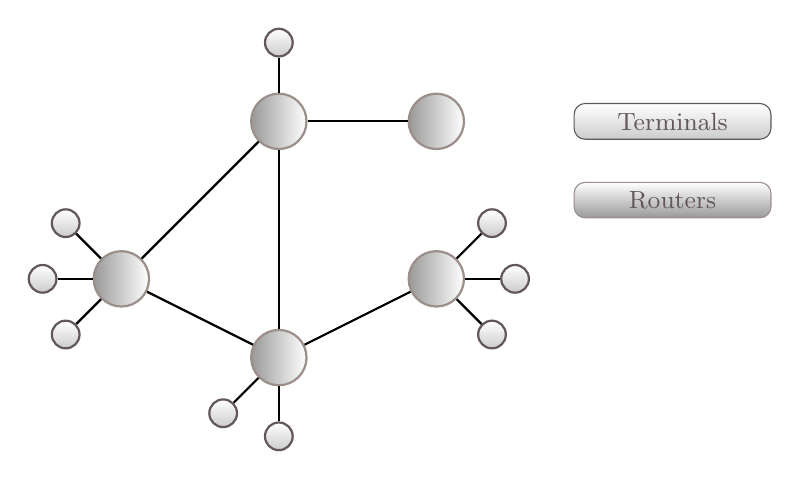
\begin{tikzpicture}[auto, thick]
  % Place super peers and connect them
  \foreach \place/\name in {{(0,-1)/a}, {(2,0)/b}, {(2,2)/c}, {(0,2)/d},
           {(-2,0)/e}}
    \node[superpeers] (\name) at \place {};
  \foreach \source/\dest in {a/b, a/d, c/d,a/e,d/e}
    \path (\source) edge (\dest);
   %
   % Place normal peers
  \foreach \pos/\i in {above left of/1, left of/2, below left of/3}
    \node[peers, \pos = e] (e\i) {};
   \foreach \speer/\peer in {e/e1,e/e2,e/e3}
    \path (\speer) edge (\peer);
   %
   \foreach \pos/\i in {above right of/1, right of/2, below right of/3}
    \node[peers, \pos =b ] (b\i) {};
   \foreach \speer/\peer in {b/b1,b/b2,b/b3}
   \path (\speer) edge (\peer);
   %
   \node[peers, above of=d] (d1){};
   \path (d) edge (d1);
   %
   \foreach \pos/\i in {below left of/1, below of/2}
   \node[peers, \pos =a ] (a\i) {};
   \foreach \speer/\peer in {a/a1,a/a2}
   \path (\speer) edge (\peer);
   %%%%%%%%
   % Legends
   \node[legendsp] at (5,1) {\small{Routers}};
   \node[legendp] at (5,2) {\small{Terminals}};
\end{tikzpicture}
